% Author: Izaak Neutelings (November, 2018)
% page 8 https://archive.org/details/StaticAndDynamicElectricity
%
%https://tex.stackexchange.com/questions/56353/extract-x-y-coordinate-of-an-arbitrary-point-on-curve-in-tikz
%
%https://tex.stackexchange.com/questions/412899/tikz-calculate-and-store-the-euclidian-distance-between-two-coordinates

\documentclass[border=3pt,tikz]{standalone}
\usepackage{amsmath} % for \dfrac
\usepackage{physics,bm}
\usepackage{tikz,pgfplots}
\usepackage[outline]{contour} % glow around text
\usetikzlibrary{angles,quotes} % for pic (angle labels)
\usetikzlibrary{decorations.markings}
\usetikzlibrary{shapes,intersections} % for path name
\tikzset{>=latex} % for LaTeX arrow head
\contourlength{1.4pt}

\usepackage{xcolor}
\colorlet{Ecol}{orange!90!black}
\colorlet{EcolFL}{orange!90!black}
\colorlet{veccol}{green!45!black}
\colorlet{EFcol}{red!60!black}
\tikzstyle{charged}=[top color=blue!20,bottom color=blue!40,shading angle=10]
\tikzstyle{darkcharged}=[very thin,top color=blue!60,bottom
color=blue!80,shading angle=10]
\tikzstyle{charge+}=[very thin,top color=red!80,bottom
color=red!80!black,shading angle=-5]
\tikzstyle{charge-}=[very thin,top color=blue!50,bottom
color=blue!70!white!90!black,shading angle=10]
\tikzstyle{darkcharged}=[very thin,top color=blue!60,bottom
color=blue!80,shading angle=10]
\tikzstyle{gauss surf}=[green!70!black,top color=green!2,bottom
color=green!80!black!70,shading angle=5,fill opacity=0.6]
\tikzstyle{gauss lid}=[gauss surf,middle color=green!80!black!20,shading
angle=40,fill opacity=0.7]
\tikzstyle{gauss dark}=[green!60!black,fill=green!60!black!70,fill opacity=0.8]
\tikzstyle{gauss line}=[green!80!black]
\tikzstyle{gauss dashed line}=[green!60!black!80,dashed,line width=0.2]
\tikzstyle{vector}=[->,thick,veccol]
\tikzstyle{normalvec}=[->,thick,blue!80!black!80]
\tikzstyle{EField}=[->,thick,Ecol]
\tikzstyle{EField dashed}=[dashed,Ecol,line width=0.6]
\tikzset{
  EFieldLine/.style={thick,EcolFL,decoration={markings,
                     mark=at position #1 with {\arrow{latex}}},
                     postaction={decorate}},
  EFieldLine/.default=0.5}
\tikzstyle{measure}=[fill=white,midway,outer sep=2]
\def\L{2.2}
\def\H{2.2}
\def\offset{2.0}
\def\W{0.30}
\def\Nx{5}
\def\Ny{5}


\colorlet{Ecol}{orange!90!black}
\colorlet{EcolFL}{orange!80!black}
\colorlet{veccol}{green!45!black}
\colorlet{EFcol}{red!60!black}
\colorlet{pluscol}{red!60!black}
\colorlet{minuscol}{blue!60!black}
\colorlet{gausscol}{green!50!black!80}
\tikzstyle{charged}=[top color=blue!20,bottom color=blue!40,shading angle=10]
\tikzstyle{charge+}=[very thin,draw=black,top color=red!80,bottom
color=red!80!black,shading angle=-5]
\tikzstyle{charge-}=[very thin,draw=black,top color=blue!50,bottom
color=blue!70!white!90!black,shading angle=10]
\tikzstyle{darkcharged}=[very thin,top color=blue!60,bottom
color=blue!80,shading angle=10]
\tikzstyle{gauss surf}=[green!40!black,top color=green!2,bottom
color=green!80!black!70,shading angle=5,fill opacity=0.6]
\tikzstyle{gauss dark}=[green!40!black,fill=green!40!black!70,fill opacity=0.8]
\tikzstyle{gauss line}=[green!40!black]
\tikzstyle{gauss dashed line}=[green!60!black!80,dashed,line width=0.2]
\tikzstyle{vector}=[->,thick,veccol]
\tikzstyle{normalvec}=[->,thick,blue!80!black!80]
\tikzstyle{EField}=[->,thick,Ecol]
\tikzstyle{EField dashed}=[dashed,Ecol,line width=0.6]
\tikzset{
  EFieldLine/.style={thick,EcolFL,decoration={markings,
                     mark=at position #1 with {\arrow{latex}}},
                     postaction={decorate}},
  EFieldLine/.default=0.5}
\tikzstyle{metal}=[top color=black!5,bottom color=black!15,shading angle=30]
\tikzstyle{measure}=[fill=green!70!black!8,midway,outer sep=0,inner sep=1]

\begin{document}


% PLANE field with electric field
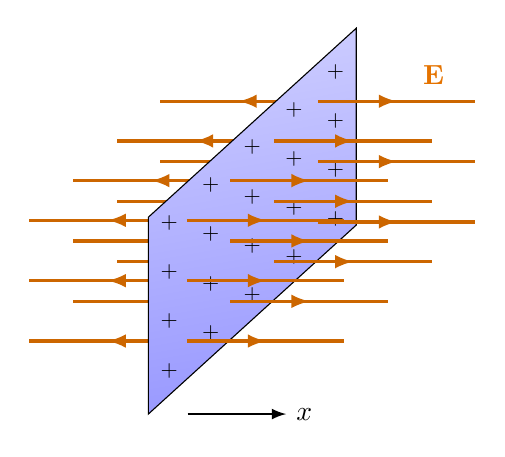
\begin{tikzpicture}[x={(1.0cm,0)},y={(0.55cm,0.5cm)},z={(0,1.0cm)}]
  \def\H{2.5}
  \def\W{4.8}
  \def\Ny{5}
  \def\Nz{4}
  \def\NEy{4}
  \def\NEz{3}
  \def\oEy{0.08*\W}
  \def\oEz{0.04*\H}
  \def\E{2}
  \coordinate (O) at (0.0,-0.5,-0.5);

  % AXES
  \draw[->,thick] (0.5,0,0) --++ (0.5*\H,0,0) node[right] {$x$};
  %\draw[->,thick] (O) --++ (0.5*\H,0,0) node[right] {$x$};
  %\draw[->,thick] (O) --++ (0,0.7*\H,0) node[right] {$y$};
  %\draw[->,thick] (O) --++ (0,0,0.5*\H) node[above] {$z$};

  % ELECTRIC FIELD back
  \foreach \i [evaluate={\y=\oEy+(\i-0.5)*(\W-2*\oEy)/\NEy;}] in {1,...,\NEy}{
    \foreach \j [evaluate={\z=\oEz+(\j-0.5)*(\H-2*\oEz)/\NEz;}] in
    {1,...,\NEz}{
      \draw[EFieldLine,very thick] (0,\y,\z) --++ (-\E,0,0);
    }
  }

  % PLANE
  \draw[charged]
    (0,0,0) --++ (0,\W,0) --++ (0,0,\H) --++ (0,-\W,0) -- cycle;
  \foreach \i [evaluate={\y=(\i-0.5)*\W/\Ny;}] in {1,...,\Ny}{
    \foreach \j [evaluate={\z=(\j-0.5)*\H/\Nz;}] in {1,...,\Nz}{
      \node[scale=0.8,rotate=0] at (0,\y,\z) {$+$};
    }
  }

  % ELECTRIC FIELD front
  \foreach \i [evaluate={\y=\oEy+(\i-0.5)*(\W-2*\oEy)/\NEy;}] in {1,...,\NEy}{
    \foreach \j [evaluate={\z=\oEz+(\j-0.5)*(\H-2*\oEz)/\NEz;}] in
    {1,...,\NEz}{
      \draw[EFieldLine,very thick] (0,\y,\z) --++ (\E,0,0);
    }
  }
  \node[Ecol] at (1.3,0.88*\W,0.88*\H) {$\vb{E}$};


\end{tikzpicture}



% PLANE field with gaussian surface
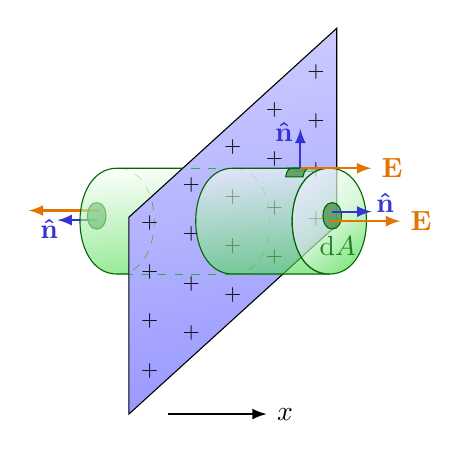
\begin{tikzpicture}[x={(1.0cm,0)},y={(0.55cm,0.5cm)},z={(0,1.0cm)}]
  \def\H{2.5}
  \def\W{4.8}
  \def\Ny{5}
  \def\Nz{4}
  \def\R{0.14*\W}
  \def\a{0.49*\H}
  \def\E{0.36*\H}
  \def\plane{(0,0,0) --++ (0,\W,0) --++ (0,0,\H) --++ (0,-\W,0) -- cycle;}
  \coordinate (O) at (0.0,-0.5,-0.5);
  \coordinate (C)  at (      0,\W/2,\H/2);
  \coordinate (ER) at (     \a,\W/2,\H/2);
  \coordinate (EL) at (-1.2*\a,\W/2-0.6*\R,\H/2+0.5*\R);
  \coordinate (TM) at (      0,\W/2,\H/2+\R);
  \coordinate (TR) at (     \a,\W/2,\H/2+\R);
  \coordinate (TL) at (-1.2*\a,\W/2,\H/2+\R);
  \coordinate (BM) at (      0,\W/2,\H/2-\R);
  \coordinate (BR) at (     \a,\W/2,\H/2-\R);
  \coordinate (BL) at (-1.2*\a,\W/2,\H/2-\R);
  \coordinate (NT) at (0.7*\a,\W/2,\H/2+\R);
  \coordinate (NR) at (\a,\W/2+0.13*\R,\H/2+0.13*\R);
  \coordinate (NL) at (-1.2*\a,\W/2-0.5*\R,\H/2-0.2*\R);
  \coordinate (NB) at (0.86*\a,\W/2-0.6*\R,\H/2-0.6*\R);

  % AXES
  \draw[->,thick] (0.5,0,0) --++ (0.5*\H,0,0) node[right] {$x$};

  % VECTORS back
  \draw[EField] (EL) --++ (-\E,0,0);
  \draw[normalvec] (EL) ++(0,-0.1*\R,-0.13*\R) --++ (-0.5,0,0) node[below
  left=-4] {$\vu{n}$};
  \draw[gauss dark]
    (EL)++(0,-0.1*\R,-0.3*\R)
      to[out=0,in=0,looseness=1.2] ++(0,0,0.5*\R)
      to[out=180,in=180,looseness=1.2] ++(0,0,-0.5*\R) -- cycle;
      %node[left=4,below=-1] {$\dd{A}$};

  % GAUSSIAN SURFACE back
  \draw[gauss dashed line] (BL) to[out=0,in=0,looseness=1.2] (TL);
  \draw[gauss surf]
    (BM) to[out=180,in=180,looseness=1.2] (TM) --
    (TL) to[out=180,in=180,looseness=1.2] (BL) -- cycle;

  % PLANE
  \draw[charged] \plane;
  \begin{scope}
    \clip \plane;
    \draw[gauss dashed line] (BM) -- (BL);
    \draw[gauss dashed line] (TM) -- (TL);
    \draw[gauss dashed line] (BL) to[out=0,in=0,looseness=1.2] (TL);
  \end{scope}
  \foreach \i [evaluate={\y=(\i-0.5)*\W/\Ny;}] in {1,...,\Ny}{
    \foreach \j [evaluate={\z=(\j-0.5)*\H/\Nz;}] in {1,...,\Nz}{
      \node[scale=0.8,rotate=0] at (0,\y,\z) {$+$};
    }
  }
  \draw[gauss dark]
    (NT) ++ (-0.12,0,0) to[out=-5,in=110] ++(0,0.12,-0.10) --++(0.22,0,0)
    to[out=110,in=-5] ++(0,-0.12,0.10) -- cycle;

  % GAUSSIAN SURFACE front
  \draw[gauss dashed line]
    (BM) to[out=0,in=0,looseness=1.2] (TM);
  \draw[gauss surf]
    (BM) to[out=180,in=180,looseness=1.2] (TM) --
    (TR) to[out=180,in=180,looseness=1.2] (BR) -- cycle;
  \draw[gauss lid]
    (BR) to[out=0,in=0,looseness=1.2] (TR) to[out=180,in=180,looseness=1.2]
    cycle;

  % DARK
  \draw[gauss dark]
    (NT) ++ (-0.12,0,0) to[out=-160,in=80] ++(0,-0.12,-0.05) --++(0.22,0,0)
    to[out=80,in=-160] ++(0,0.12,0.05) -- cycle;
  \draw[gauss dark]
    (ER)++(0,0.1*\R,-0.2*\R)
      to[out=0,in=0,looseness=1.2] ++(0,0,0.5*\R)
      to[out=180,in=180,looseness=1.2] ++(0,0,-0.5*\R) -- cycle
      node[right=2,below=-1] {$\dd{A}$};

  % ELECTRIC FIELD
  \draw[EField] (ER) --++ (\E,0,0) node[right] {$\vb{E}$};
  \draw[EField] (NT) --++ (\E,0,0) node[right] {$\vb{E}$};

  % VECTORS
  \draw[normalvec] (ER) ++(0,0.1*\R,0.13*\R) --++ (0.5,0,0)
  node[above=3,right=-2] {$\vu{n}$};
  \draw[normalvec] (NT) --++ (0,0,0.5) node[below=1,left=-1] {$\vu{n}$};
  %\draw[normalvec] (NB) --++ (0,-0.35,-0.25) node[below right=-2] {$\vu{n}$};


\end{tikzpicture}



% POINT CHARGE +1
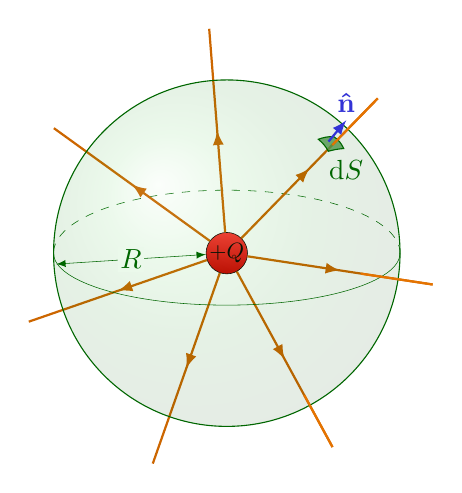
\begin{tikzpicture}
  \def\N{7}
  \def\R{2.2}
  \def\r{0.8}

  % SPHERE BACK
  \begin{scope}
    \clip (-\R,0) rectangle ++(2*\R,\R);
    \draw[gauss line,very thin,dashed]
      (0,0) ellipse ({\R} and {\r});
  \end{scope}

  % CHARGES
  \node[charge+,scale=0.8,circle,inner sep=0.27] (C) at (0,0) {$+Q$};

  % FIELD LINES
  \path[name path=ell](0,0) ellipse ({0.78*\R} and {\R});
  \foreach \i [evaluate={\ang=-8+\i*360/\N;}] in {1,...,\N}{
    %\message{Eline\i^^J}
    \draw[EFieldLine,name path global/.expanded=Eline\i] (C) --
    ({1.2*\R*cos(\ang)},{1.3*\R*sin(\ang)}) coordinate (E\i);
    %(\ang:1.3*\R)
  }

  % SPHERE
  \draw[gauss line,ball color=green!70!black,fill opacity=0.1]
    (0,0) circle (\R);
  \begin{scope}
    \clip (-\R,0) rectangle ++(2*\R,-\R);
    \draw[gauss line,very thin]
      (0,0) ellipse ({\R} and {0.3*\R});
  \end{scope}
  \draw[<->,gauss line,very thin]
    (C) -- (190:{\R} and {\r}) node[measure] {$R$};
    %{\contour{green!70!black!7}{$R$}};

  % VECTOR
  \draw[gauss dark,name intersections={of={Eline1} and ell,name=ES1}]
    (ES1-1) ++ (-0.081*\R,0.033*\R) to[out=20,in=180] ++(10:0.09*\R)
                                    to[out=-35,in=115] ++(-50:0.09*\R)
                                    to[out=185,in=15] ++(190:0.09*\R)
                                    to[out=120,in=-40] cycle; %node[left]
                                    %{$\dd{A}$};
  \node[green!40!black,right=5,below=2] at (ES1-1) {$\dd{S}$};
  \foreach \i [evaluate={\angle=8+\i*360/\Nx;}] in {1,6,7}{
    \draw[EField,-,name intersections={of={Eline\i} and ell,name=ES\i}]
    (ES\i-1) -- (E\i);
  }
  \draw[normalvec] (ES1-1) ++ (138:0.03*\R) --++ (50:0.16*\R) node[above=-1]
  {$\vu{n}$};

\end{tikzpicture}



% SOLID CHARGED SPHERE 2D
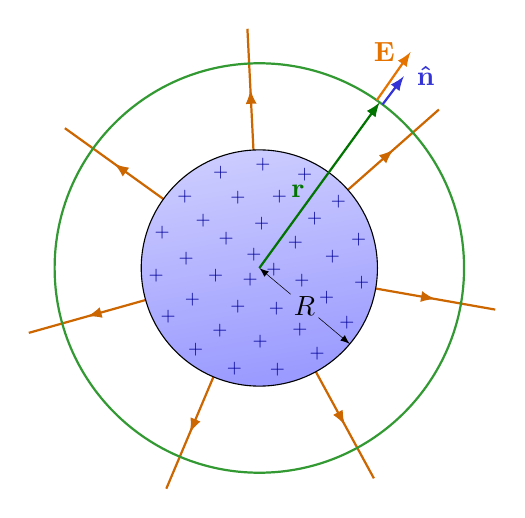
\begin{tikzpicture}
  \def\NE{7}
  \def\NQ{4}
  \def\R{1.5}
  \def\r{2.6}

  % FIELD LINES
  \foreach \i [evaluate={\ang=-10+\i*360/\NE;}] in {1,...,\NE}{
    \draw[EFieldLine] (\ang:\R) -- (\ang:1.17*\r);
  }

  % SPHERE
  \draw[charged]
    (0,0) circle (\R);
  \draw[gausscol,thick]
    (0,0) circle (\r);

  % CHARGES
  \foreach \i [evaluate={\rc=(\i-0.5)*\R/\NQ; \N=-1+4*\i;}] in {1,...,\NQ}{
    \foreach \j [evaluate={\ang=-8*\i+\j*360/\N;}] in {1,...,\N}{
      \node[minuscol,scale=0.7] at (\ang:\rc) {$+$};
    }
  }

  % VECTORS
  \node[inner sep=1] (R) at (-40:\R/2) {$R$};
  \draw[<-,very thin] (0,0) -- (R);
  \draw[->,very thin] (R) -- (-40:\R);
  \draw[vector] (0,0) -- (54:\r) node[pos=0.46,left=0] {$\vb{r}$};
  \draw[EField] (55:\r) --++ (55:0.5*\R) node[left=2] {$\vb{E}$};
  \draw[normalvec] (53:\r) --++ (53:0.3*\R) node[right=1] {$\vu{n}$};

\end{tikzpicture}


% SOLID CHARGED SPHERE 2D
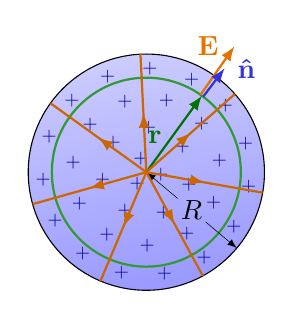
\begin{tikzpicture}
  \def\NE{7}
  \def\NQ{4}
  \def\R{1.5}
  \def\r{1.2}



  % SPHERE
  \draw[charged]
    (0,0) circle (\R);
  \draw[gausscol,thick]
    (0,0) circle (\r);

  % CHARGES
  \foreach \i [evaluate={\rc=(\i-0.5)*\R/\NQ; \N=-1+4*\i;}] in {1,...,\NQ}{
    \foreach \j [evaluate={\ang=-8*\i+\j*360/\N;}] in {1,...,\N}{
      \node[minuscol,scale=0.7] at (\ang:\rc) {$+$};
    }
  }

  % VECTORS
  \node[inner sep=1] (R) at (-40:\R/2) {$R$};
  \draw[<-,very thin] (0,0) -- (R);
  \draw[->,very thin] (R) -- (-40:\R);
  \draw[vector] (0,0) -- (54:\r) node[pos=0.46,left=0] {$\vb{r}$};
  \draw[EField] (55:\r) --++ (55:0.5*\R) node[left=2] {$\vb{E}$};
  \draw[normalvec] (53:\r) --++ (53:0.3*\R) node[right=1] {$\vu{n}$};

  % FIELD LINES
  \foreach \i [evaluate={\ang=-10+\i*360/\NE;}] in {1,...,\NE}{
    \draw[EFieldLine] (\ang:0) -- (\ang:\R);
  }

\end{tikzpicture}


% HOLLOW CHARGED SPHERE 2D
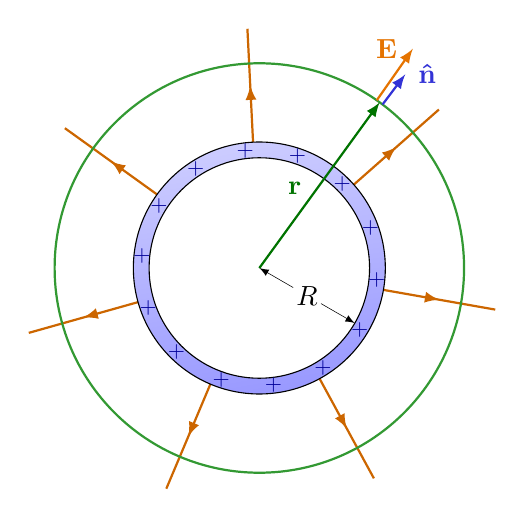
\begin{tikzpicture}
  \def\NE{7}
  \def\NQ{14}
  \def\Rin{1.40}
  \def\Rout{1.60}
  \def\r{2.6}

  % FIELD LINES
  \foreach \i [evaluate={\ang=-10+\i*360/\NE;}] in {1,...,\NE}{
    \draw[EFieldLine] (\ang:\Rout) -- (\ang:1.17*\r);
  }

  % SPHERE
  \draw[charged,even odd rule]
    (0,0) circle (\Rin) circle (\Rout);
  \draw[gausscol,thick]
    (0,0) circle (\r);

  % CHARGES
  \foreach \i [evaluate={\ang=-6+\i*360/\NQ;}] in {1,...,\NQ}{
    \node[minuscol,scale=0.8] at (\ang:{(\Rin+\Rout)/2}) {$+$};
  }

  % VECTORS
  \node[inner sep=1] (R) at (-30:\Rin/2) {$R$};
  \draw[<-,very thin] (0,0) -- (R);
  \draw[->,very thin] (R) -- (-30:\Rin);

  \draw[vector] (0,0) -- (54:\r) node[pos=0.48,left=2] {$\vb{r}$};
  \draw[EField] (55:\r) --++ (55:0.5*\Rout) node[left=2] {$\vb{E}$};
  \draw[normalvec] (53:\r) --++ (53:0.3*\Rout) node[right=1] {$\vu{n}$};

\end{tikzpicture}




\end{document}